\section{Uma Nova Linguagem}

\begin{frame}[fragile]{Rust}
\begin{figure}[ht!]
  \centering
%   \includegraphics[scale=0.08]{images/rust.png}
  \includesvg[inkscapelatex=false, scale=0.30]{images/origin_rust.svg}
\end{figure}
% \begin{itemize}
%     \item \textbf{moz://a} Mozilla Foundation
%     \item \textbf{Open Source} https://github.com/rust-lang/rust
%     \item \textbf{Star} 38.651  \textbf{Fork} 6.011 \textbf{Contributors} 2.457
% \end{itemize}
\begin{center}
    O que me levou a me interessar por \textbf{Rust}?
\end{center}

\begin{center}
    https://www.rust-lang.org
\end{center}{}
\end{frame}

\begin{frame}[fragile]{O que me levou a me interessar por Rust?}
\begin{center}
\begin{itemize}
    \item \textbf{moz://a} Mozilla Foundation
    \begin{itemize}
        \item \textbf{Star} 38.651  \textbf{Fork} 6.011 \textbf{Contributors} 2.457
    \end{itemize}{}
    \item \textbf{Paradigmas:}
    \begin{itemize}
        \item Programação genérica, Concorrente, Estruturado e funcional
    \end{itemize}{}
    \item \textbf{Segurança}
    \begin{itemize}
        \item Segurança de memória sem \textbf{Garbage Collector} ou \textbf{Runtime}.
        \item Concorrência sem disputa de dados.
    \end{itemize}
    \item \textbf{Performance}
    \begin{itemize}
        \item Performance comparável a da linguagem \textbf{C}
        \item Abstração sem \textbf{overhead}.
    \end{itemize}{}
    \item \textbf{Casos de sucesso}
\end{itemize}
\end{center}
\begin{center}
    \begin{figure}[ht!]
  \centering
  \includegraphics[scale=0.6]{images/cases.png}
\end{figure}
\end{center}{}
\end{frame}

\begin{frame}[fragile]{O que me levou a me interessar por Rust?}
\begin{figure}[ht!]
  \centering
  \includegraphics[scale=0.4]{images/webassembly.png}
\end{figure}
\begin{center}
\small{Possui suporte nativo ao \textbf{WebAssembly}}
\end{center}
\begin{center}
\small{https://webassembly.org/}
\end{center}
\end{frame}

\begin{frame}[fragile]{O que me levou a me interessar por Rust?}
\begin{figure}[ht!]
  \centering
  \includegraphics[scale=0.6]{images/n-body.jpg}
\end{figure}
\begin{center}
\small{A simulação N-body permite calcular a evolução gravitacional de uma galáxia}
\end{center}
\end{frame}

\begin{frame}[fragile]{O que me levou a me interessar por Rust?}
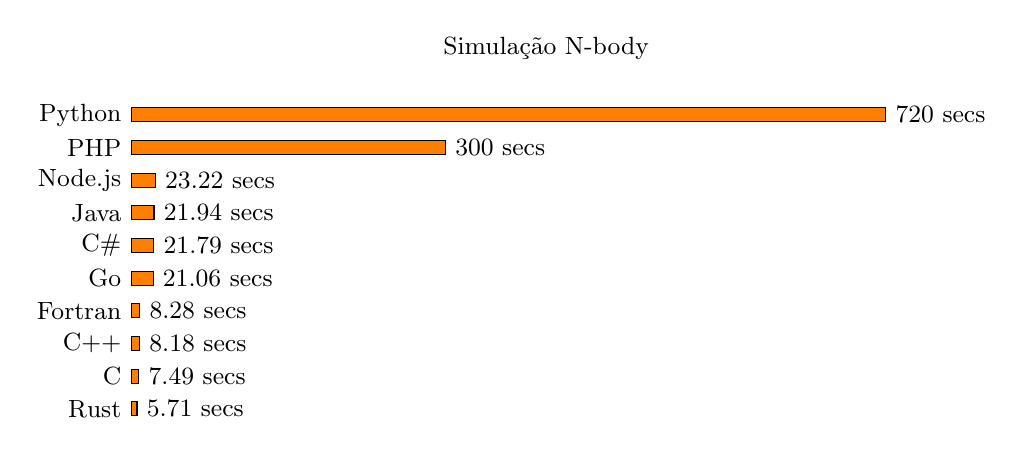
\begin{tikzpicture}[font=\small]
\pgfplotsset{
    width=\textwidth,
    height=0.5\textwidth
}
\begin{axis}
[
    xbar,
    title = Simulação N-body,
    y axis line style = { draw=none },
    axis x line = none,
    tickwidth = 0pt,
    nodes near coords,
    nodes near coords={\pgfmathprintnumber[precision=1000]\pgfplotspointmeta \ secs},
    xmin=0,
    ytick distance=1,
    symbolic y coords = { Rust, C, C++, Fortran, Go, C\#, Java, Node.js, PHP, Python},
]
    \addplot[
      fill=orange, 
      bar width=5pt,
    ] coordinates { 
    (5.71,Rust)
    (7.49,C)
    (8.18,C++)
    (8.28,Fortran)
    (21.06,Go)
    (21.79,C\#)
    (21.94,Java)
    (23.22,Node.js)
    (300.0,PHP)
    (720,Python)
    };
  \end{axis}
\end{tikzpicture}
\begin{center}
\small{Simular a evolução gravitacional de 4 planetas com N = 50.000.000}
\small{https://benchmarksgame-team.pages.debian.net/benchmarksgame/}
\end{center}
\end{frame}

% Ownership
\begin{frame}[fragile]{Que é Ownership}
\lstset{language=Rust, style=boxed}
\begin{lstlisting}
fn main() {
    let s1 = String::from("Hello World");

    let _s2 = s1; // <= Ownership

    println!("{}", s1);
}
\end{lstlisting}

\begin{lstlisting}
error[E0382]: use of moved value: `s1`
\end{lstlisting}
\begin{itemize}  
\item Rust a memória é gerenciada através de um sistema de posse
\item Gera  \textbf{código nativo} inteligente de desalocação.
\item Sem os \textbf{memory-leaks} das linguagens não gerenciadas. 
\item Sem os \textbf{overheads} de processamento causados pelos  \textbf{GCs}. 
\end{itemize}
\end{frame}

\begin{frame}[fragile]{Ownership - Clone ou Referência}
\lstset{language=Rust, style=boxed}
\begin{lstlisting}
// Ownership
fn main() {
    let s1 = String::from("Hello World");

    // Clona s1 para _s2
    let _s2 = s1.clone();
    
    // OU
    
    // referencia ao valor s1, mas nao o possui.
    let _s2 = &s1; 

    println!("{}", s1);
}
\end{lstlisting}
\end{frame}

% Variáveis são imutáveis por padrão;
\begin{frame}[fragile]{Variáveis e Mutabilidade}
\lstset{language=Rust, style=boxed}
\begin{lstlisting}
fn main() {
    let x = 5;
    
    x = 6;

    println!("O valor de x e {}", x);
}
\end{lstlisting}
\begin{lstlisting}
error[E0384]: cannot assign twice to immutable variable `x`
\end{lstlisting}
\begin{itemize}
    \item Em Rust, por padrão, as variáveis são \textbf{imutáveis}.
    \item O compilador não deixa atribuir mais de uma vez à variável imutável \textbf{x}.
\end{itemize}
\end{frame}

\begin{frame}[fragile]{Variáveis e Mutabilidade - mut}
\lstset{language=Rust, style=boxed}
\begin{lstlisting}
fn main() {
    let mut x = 5;
    
    x = 6;

    println!("O valor de x e {}", x);
}
\end{lstlisting}

\begin{lstlisting}
$ cargo run

O valor de x e: 5
O valor de x e: 6
\end{lstlisting}
\begin{itemize}
    \item A palavra chave \textbf{mut} autoriza a mudar o valor 5 contido em x para 6.
\end{itemize}{}
\end{frame}

% Shadowing
\begin{frame}[fragile]{Shadowing}
\lstset{language=Rust, style=boxed}
\begin{lstlisting}
fn main() {
    let x = 5;
    
    let x = x + 1;
    
    let x = x * 2;

    println!("O valor de x e: {}", x);
}
\end{lstlisting}

\begin{lstlisting}
$ cargo run

O valor de x e: 12
\end{lstlisting}
\begin{itemize}
    \item Você pode declarar uma nova variável com o mesmo nome de uma variável anterior, e a nova variável sombreia a variável anterior.
\end{itemize}
\end{frame}

% Operador Match
\begin{frame}[fragile]{Operador match}
\lstset{language=Rust, style=boxed}
\begin{lstlisting}
fn fibonacci(n: i32) -> u64 {
    match n {
        0 => panic!("zero is not argument!"),
        1 | 2 => 1,
        50 => 12586269025,
        100 => 354224848179261915075,
        _  => fibonacci(n - 1) + fibonacci(n - 2)
    }
}
\end{lstlisting}
\begin{itemize}
    \item O operador \textbf{match} nos permite comparar um valor com uma série de padrões e executar um código com base no padrão que casar.
\end{itemize}
\end{frame}

% Tratamento de Erros
\begin{frame}[fragile]{Tratamento de Erros}
\lstset{language=Rust, style=boxed}
\begin{lstlisting}
enum Result<T, E> {
    Ok(T),
    Err(E),
}
\end{lstlisting}

\begin{itemize}
    \item Rust agrupa erros em duas categorias principais:
\begin{itemize}
    \item \textbf{recuperáveis} - Erros recuperáveis são situações em que é razoável reportar o problema ao usuário.
    \item \textbf{irrecuperáveis} - Erros irrecuperáveis são sempre sintomas de bugs.
\end{itemize}
\end{itemize}

\end{frame}

\begin{frame}[fragile]{Entrar em panic! ou Não Entrar em panic!}
\lstset{language=Rust, style=boxed}
\begin{lstlisting}
use std::fs::File;

fn main() {
    let f = File::open("hello.txt");

    let f = match f {
        Ok(file) => file,
        Err(error) => {
            panic!("fail: {:?}", error)
        },
    };
}
\end{lstlisting}
\begin{itemize}
    \item Em algumas situações é mais apropriado escrever código que entra em pânico em vez de retornar um Result.
\end{itemize}

\end{frame}
